\section{AV security attacks on sensors}

\subsection{Global Positioning System}
    To bypass the difficulties of get GPS data, the count of satellites with public domain is increased so everyone can easily access these data. Because of this an adversary can mislead or manipulate data to provide the wrong directions, to control the routing of the 
    vehicle or to make the vehicle crash [10].
    \newline
    GPS jamming is an attack where the adversary temporarily blocks GPS signals by sending more powerful signal in the same frequency. This type of attack is really effective on AV because to perfectly locate and navigate, autonomous vehicles need to use GPS data with great accuracy [11]. 
    GPS spoofing is an attack where an adversary forges counterfeit GPS signals and send them to the target as valid ones. 
    \newline    
    GPS spoofing relies on GPS jamming to block valid signals before sending the counterfeited ones. GPS spoofing is really effective on AVs for the same reasons  as  GPS  jamming.  Public  GPS  is  not  designed  to  be secure because of its public nature. The only countermeasure to GPS spoofing is authentication, achievable through proper encryption [12].
    \newline    
    Given the fact that GPS are programmed to receive the stronger signals, the adversary  just by sending a strong unrealistic signal can gradually modify the position of the vehicle from the desired target [13]. 
    \newline    
    To prevent this type of attacks researchers developed many simple validation mechanisms that can be put in place. For example monitoring identification codes, satellite signals, and the use of time intervals can help detect spoofing and jamming attempts. 
    \newline    
    In [14]  is detailed how the observed signal strength would be expected to be around 163 decibel watts so a solution could be to block signal with higher frequencies. However, if the attack is sufficient smart enough to appear genuine, these validation checks will fail and the GPS device will be manipulated. 
    \newline
    Q. Yang et al. in [15] combined antijamming and antispoofing algorithm for a GPS receiver based on an antenna array. In their method, the jamming is eliminated by subspace projection, and then a compressed sensing framework is adopted to obtain the direction of arrival (DOA) of the despreading satellite navigation signal and detect the spoofing signal. According to the DOA of the authentic and spoofing signals, the receiver uses adaptive multibeamforming to concurrently achieve the undistorted reception of the authentic satellite signal and the suppression of the spoofing.
    \newline
    However, in our knowledge, a good and realistic solution to prevent these attacks has not yet been found. The only way to avoid GPS Jamming and GPS Spoofing is to implement a military-grade cryptographic.
    
\subsection{Light Detection and Ranging (LiDAR)}
    LiDAR is a type of range-finding sensor that emits light pulses and measures the time it takes to reflect off a distant surface, called a ping. These laser pulses are commonly bounced off of a spinning mirror thousands of times per second, creating a scan of laser pulses. When the original pulse is received more than once, these additional pulses received are called echoes. Echoes are useful to detect objects under almost any weather condition [16].
    \newline
    Relaying signal attack could be seen as an extension of the replay attack where aims is to relay the original signal sent from the target vehicle LiDAR from another position to create fake echos, and eventually move objects from their real position [17]. J. Petit et al. demonstrate that using only two transceivers at the modest cost of 45\$ is possible to perform this attack. Basically the first transceiver is a photodetector sensitive to the LiDAR wavelength (905nm) that produce in output a voltage signal that corresponds to the intensity of the pulse sent by the LiDAR. That output is then sent to the second transceiver, which uses a laser to emit a pulse in return.
    \newline
    Spoofing signal attack is an extension of the previous one and with this one an adversary, by sending a signal of the same frequency to the scanner, can create fake objects. LiDAR typically listen for incoming reflection for at least \SI{1.33}{\micro\second}. To successfully inject signals into the LiDAR, the counterfeit signal should arrive within this window. The earlier the LiDAR receives the signal, the closer it will be to the LiDAR.
    Therefore, if the attacker delays the original signal before it relays it, it can control the position of the objects.
    \newline
    These attacks makes an AV to move slowly or stop and doing this in a highway could also result in the cost of lives [17-20].
    \newline
    \begin{figure}
        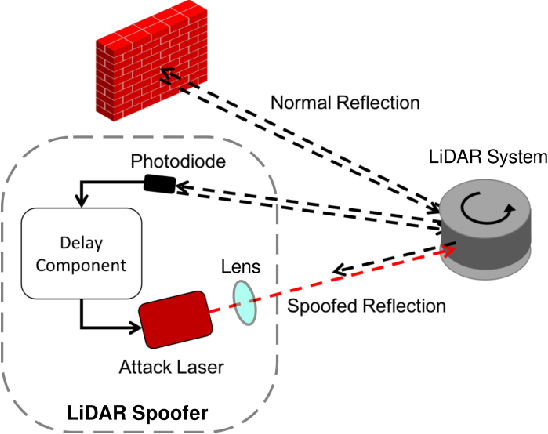
\includegraphics[width=9cm]{./files/lidarspoof.png}
        \caption{Relaying and Spoofing signal attacks on LiDAR.}
    \end{figure}
    Because the attacker need to be synchronized with the pulse interval of LiDAR few possible countermeasures could be:
    \begin{itemize}
        \item non-predictability skip of certain pulses, in this scenario LiDAR skip a pulse but it still listen for incoming pulses. If it notice a response this may indicate that an attacks is going on;
        \item shortening the pulse period of LiDAR we drastically reduce the attack window on the sensor but decreasing the ping period means decrease the working range of the sensor [17].
    \end{itemize}
    What i can understand form these attacks is that LiDAR pulses are not encoded. In our knowledge would be interesting to try adding an encoding of lidar pulses to prevent these attacks.
    
\subsection{Camera}
    A camera is an optical device that can perceive the world as a digital video signal. Cameras are frequently found in AVs for many applications; they are used for lane detection [21], traffic sign recognition [22], headlight detection [23], etc. 
    \newline
    A really effective attack on this sensor is to blind it fully or partially, by emitting light. Failing to detect objects such as speed limit signage or traffic light can put passengers is serious trouble [17]. According to an MIT Technology Review, the Google Driverless Car is susceptible to this problem where low sunlight is able to blind the vehicle’s cameras [24].
    \newline
    Another attack, similar to the previous one, presented in [17] consists on influencing the auto controls in the period before the image recovers and stabilizes after high exposure to a light source. The longer it takes to stabilize to the new environmental conditions, the longer the car is vulnerable to objects it cannot detect. This attack is limited to front/rear/side attack, because it assumes that the attacker continuously switches the light on and off. 
    \newline
    Possible countermeasures are to introduce multiple cameras that provide the same image so the attacker has to put more effort into the attack to blind all cameras at the same time. Integrating a removable near-infrared-cut filter, a technique that is available on security cameras, can filter near-infrared light on request. Another option is to use photochromic lenses. These types of lenses can change color to filter out specific types of light [17]. 

\subsection{Inertial Measurement Units (IMU)}
    IMU is the combination of the Gyroscope and Accelerometers which provides the data of velocity, acceleration, and orientation of the vehicle. They also monitor the change in the environmental dynamics like the gradient. The data provided by the sensors can be modified to not recognize the gradient of the road. 
    \newline
    Karl Koscher et al. in [25] developed CarShark tool to observe data traffic on CAN bus system, performs a detailed packet analysis and modification of packets - simulating a man-in-the-middle attack on the CAN network - and observing the effect on the vehicle. As result they were able to modify sensor’s value through changing data packet.
    \newline
    A possible mitigation system could be to use an encrypted communication on the vehicle’s communication network. Another one could be the use of additional sensors to provide a secondary source of measurement like the GPS. For example, data taken from GPS can help to determine if the vehicle is located on steep gradient.
